\documentclass[aps,prb,twocolumn,superscriptaddress,floatfix,longbibliography]{revtex4-2}

\usepackage[utf8]{inputenc}
\usepackage[spanish]{babel}
\usepackage{graphicx}
\usepackage{amsmath}
\usepackage{subcaption}
\usepackage{wrapfig} 
\usepackage[export]{adjustbox}

\usepackage{amsmath,amssymb} % math symbols
\usepackage{bm} % bold math font
\usepackage{graphicx} % for figures
\usepackage{comment} % allows block comments
\usepackage{textcomp} % This package is just to give the text quote '
\usepackage{listings} %para agregar código

%\usepackage{ulem} % allows strikeout text, e.g. \sout{text}

\usepackage[spanish]{babel}

\usepackage{enumitem}
\setlist{noitemsep,leftmargin=*,topsep=0pt,parsep=0pt}

\usepackage{xcolor} % \textcolor{red}{text} will be red for notes
\definecolor{lightgray}{gray}{0.6}
\definecolor{medgray}{gray}{0.4}

\usepackage{hyperref}
\hypersetup{
colorlinks=true,
urlcolor= blue,
citecolor=blue,
linkcolor= blue,
bookmarks=true,
bookmarksopen=false,
}

% Code to add paragraph numbers and titles
\newif\ifptitle
\newif\ifpnumber
\newcounter{para}
\newcommand\ptitle[1]{\par\refstepcounter{para}
{\ifpnumber{\noindent\textcolor{lightgray}{\textbf{\thepara}}\indent}\fi}
{\ifptitle{\textbf{[{#1}]}}\fi}}
%\ptitletrue  % comment this line to hide paragraph titles
%\pnumbertrue  % comment this line to hide paragraph numbers

% minimum font size for figures
\newcommand{\minfont}{6}

% Uncomment this line if you prefer your vectors to appear as bold letters.
% By default they will appear with arrows over them.
% \renewcommand{\vec}[1]{\bm{#1}}

%Cambiar Cuadros por Tablas y lista de...
%\renewcommand{\listtablename}{Índice de tablas}
\renewcommand{\tablename}{Tabla}
\renewcommand{\date}{Fecha}

% \graphicspath{ {C:/Users/lupam/Mi unidad/Pablo Chehade/Instituto Balseiro (IB)/Laboratorio Avanzado/Informe/V5/Figures} } %Para importar imagenes desde una carpeta


\lstset{
  basicstyle=\ttfamily\small,
  breaklines=true,
  frame=single,
  numbers=left,
  numberstyle=\tiny,
  keywordstyle=\color{blue},
  commentstyle=\color{green},
  stringstyle=\color{red},
} %Configuración para el bloque de código


\usepackage[bottom]{footmisc} %para que las notas al pie aparezcan en la misma página



\begin{comment}

%Comandos de interes:

* Para ordenar el documento:
\section{Introducción}
\section{\label{sec:Formatting}Formatting} %label para luego hacer referencia a esa sección

\ptitle{Start writing while you experiment} %pone nombre y título al documento dependiendo de si en el header están los comandos \ptitletrue y \pnumbertrue

* Ecuaciones:
\begin{equation}
a^2+b^2=c^2 \,.
\label{eqn:Pythagoras}
\end{equation}

* Conjunto de ecuaciones:
\begin{eqnarray}
\label{eqn:diagonal}
\nonumber d & = & \sqrt{a^2 + b^2 + c^2} \\
& = & \sqrt{3^2+4^2+12^2} = 13
\end{eqnarray}

* Para hacer items / enumerar:
\begin{enumerate}
  \item
\end{enumerate}

\begin{itemize}
  \item
\end{itemize}

* Figuras:
\begin{figure}[h]
    \includegraphics[clip=true,width=\columnwidth]{pixel-compare}
    \caption{}
     \label{fig:pixels}
\end{figure}

* Conjunto de figuras:
(no recuerdo)


* Para hacer referencias a fórmulas, tablas, secciones, ... dentro del documento:
\ref{tab:spacing}

* Para citar
Elementos de .bib
\cite{WhitesidesAdvMat2004}
url
\url{http://www.mendeley.com/}\\

* Agradecimientos:
\begin{acknowledgments}
We acknowledge advice from Jessie Zhang and Harry Pirie to produce Fig.\ \ref{fig:pixels}.
\end{acknowledgments}

* Apéndice:
\appendix
\section{\label{app:Mendeley}Mendeley}

* Bibliografía:
\bibliography{Hoffman-example-paper}

\end{comment}



\begin{document}

% Allows to rewrite the same title in the supplement
\newcommand{\mytitle}{Estadística de trenes de spikes}

\title{\mytitle}

\author{Pablo Chehade \\
    \small \textit{pablo.chehade@ib.edu.ar} \\
    \small \textit{Redes Neuronales, Instituto Balseiro, CNEA-UNCuyo, Bariloche, Argentina, 2023} \\}
    
    
    
\maketitle

En el ámbito de la neurociencia, el estudio de la actividad eléctrica neuronal es esencial para comprender los mecanismos subyacentes al procesamiento de la información en el cerebro. Una herramienta fundamental en este estudio es el análisis estadístico de los spikes o potenciales de acción. En este trabajo, se analizaron datos experimentales obtenidos por Ariel Rokem a través de electrodos intracelulares en un receptor acústico de un saltamontes. Estos datos comprenden la envolvente de una onda sonora presentada al animal y la respuesta neuronal correspondiente en forma de spikes. Se registraron 128 series de datos, cada una correspondiente a la respuesta neuronal ante el mismo estímulo. Todas las series de datos tienen como dato inicial un spike, el cual fue ignorado en el análisis.

\section{Distribución de intervalos entre spikes}

\begin{figure}[h]
  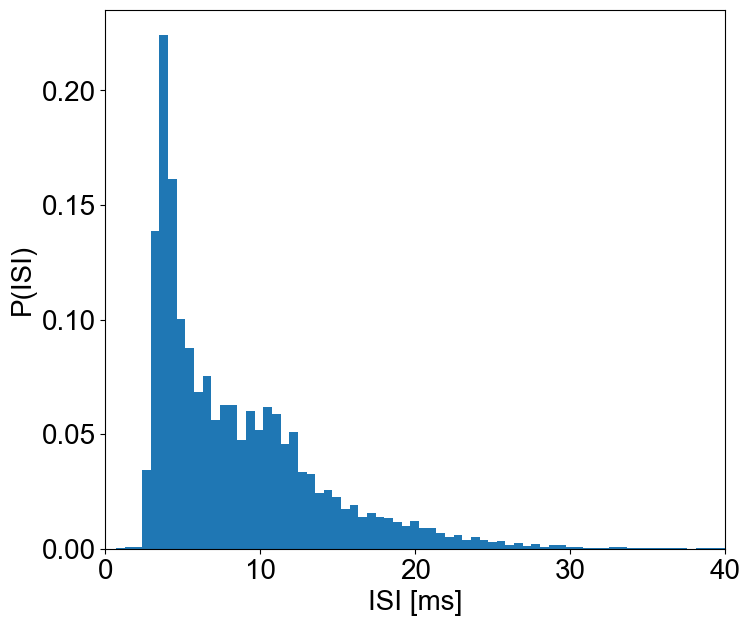
\includegraphics[clip=true,width=0.8\columnwidth]{ISI_histogram.png}
  \caption{Aproximación de la distribución de intervalos entre spikes P(ISI) de la neurona.}
   \label{fig:ISI_histogram}
\end{figure}

A partir de los datos de spikes, se determinaron los intervalos entre spikes (Inter Spike Interval o "ISI" por sus siglas en inglés). Estos intervalos se definen como la diferencia temporal entre spikes consecutivos. A continuación, se construyó un histograma de estos intervalos que, normalizado, constituye una aproximación a la distribución de intervalos P(ISI) de la neurona, como se muestra en la figura \ref{fig:ISI_histogram}. La ausencia de valores cercanos a cero refleja el período refractario de la neurona, un intervalo post-spike durante el cual es improbable que se genere otro spike. Para valores elevados de ISI, la distribución muestra un decaimiento que se asemeja a una función exponencial decreciente. En valores intermedios de ISI, se observa un comportamiento atípico con un pico seguido de una meseta de valor aproximadamente constante.

Además, se puede hacer una caracterización cuantitativa de la distribución. La media de la distribución es $\langle \mathrm{ISI} \rangle = 8.496$ ms y la desviación estándar, $\sigma_{\mathrm{ISI}} = 5.663$ ms, resultando en un Coeficiente de Variabilidad $\mathrm{CV} = \langle \mathrm{ISI} \rangle / \sigma_{\mathrm{ISI}} =  0.667$.

\section{Distribución del número de spikes}

\begin{figure}[h]
  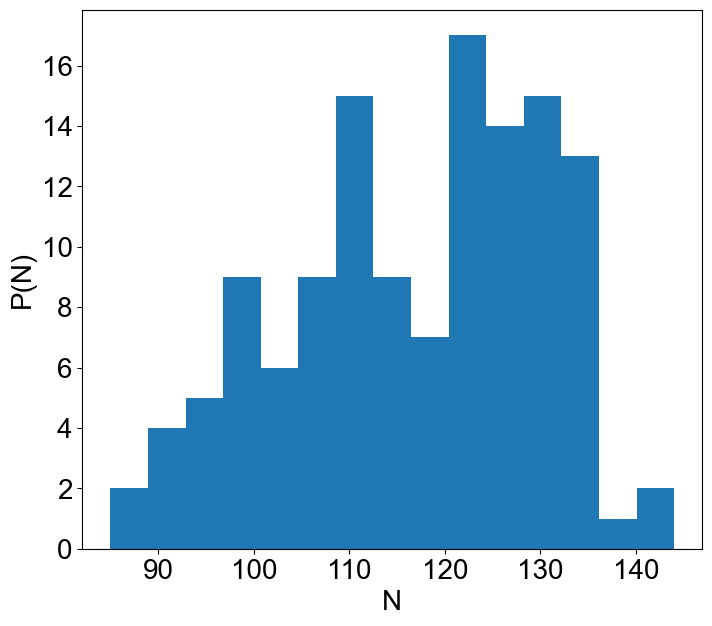
\includegraphics[clip=true,width=0.8\columnwidth]{N_histogram.png}
  \caption{Aproximación la distribución del número de spikes P(N) en cada realización.}
   \label{fig:N_histogram}
\end{figure}


Otro modo de caracterizar la respuesta neuronal es estudiando la variación de la respuesta ante el mismo estímulo. Para tal fin se contabilizó el número total de spikes, N, en cada realización y, mediante un histograma, se estimó la probabilidad P(N) de obtener N spikes en una realización. Los resultados se muestran en la figura \ref{fig:N_histogram}. Se observa que existe una variabilidad en el número de spikes generados en respuesta al mismo estímulo. Esto podría deberse a que el estímulo sonoro no es el único estímulo que recibe la neurona. Hay otros procesos que ocurren en el cerebro o en las neuronas cercanas que también la están estimulando y, por lo tanto, cambiando su respuesta. Cuantitativamente, la media de esta distribución es $\langle \mathrm{N} \rangle = 117$, mientras que la desviación estándar es $\sigma_{\mathrm{N}} = 13.5$. De este modo, el Factor de Fano $\mathrm{F}$ es $\mathrm{F} =  \sigma_\mathrm{N}^2/\langle \mathrm{N} \rangle = 1.6$.

En base a los resultados obtenidos, se puede determinar si el proceso de generación de spikes es del tipo renewal. En estos procesos se cumple la relación $\mathrm{F} = \mathrm{CV}^2$. Sin embargo, en este análisis F es 1.6, mientras que $\mathrm{CV}^2$ es 0.444. Por lo tanto, el proceso no es del tipo renewal. Esta discrepancia es coherente con la naturaleza de las neuronas reales, donde los ISI no son eventos independientes ya que la neurona tiene "memoria" del comportamiento previo.



\begin{figure}[h]
  \centering
  \begin{subfigure}[b]{0.35\textwidth}
      \centering
      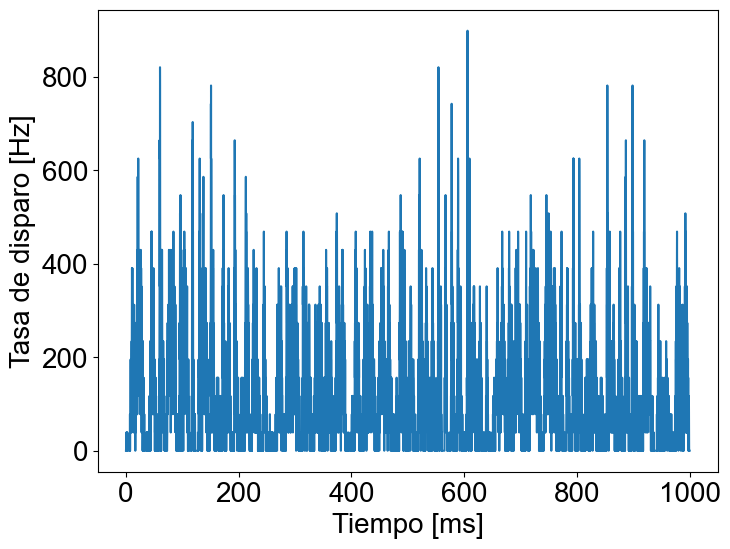
\includegraphics[width=\textwidth]{tasa_de_disparo_2.png}
      \caption{\label{fig:tasa_de_disparo_2}}
  \end{subfigure}
  \hfill
  \begin{subfigure}[b]{0.35\textwidth}
      \centering
      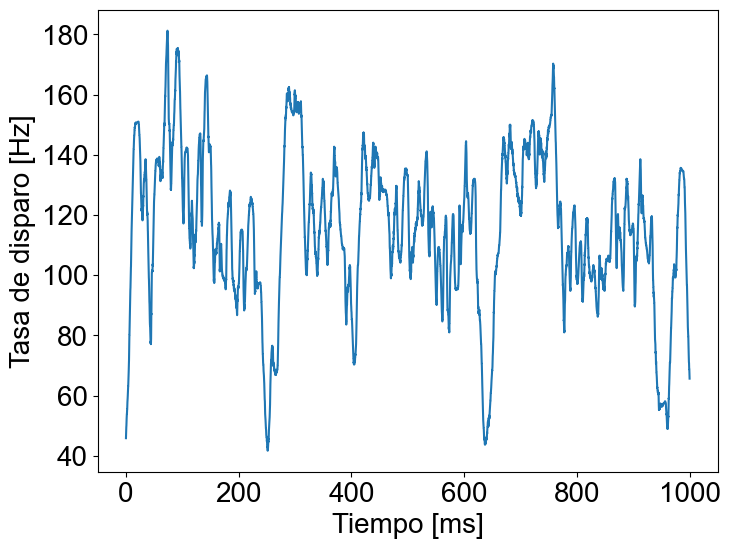
\includegraphics[width=\textwidth]{tasa_de_disparo_300.png}
      \caption{\label{fig:tasa_de_disparo_300}}
  \end{subfigure}
  \hfill
  \begin{subfigure}[b]{0.35\textwidth}
      \centering
      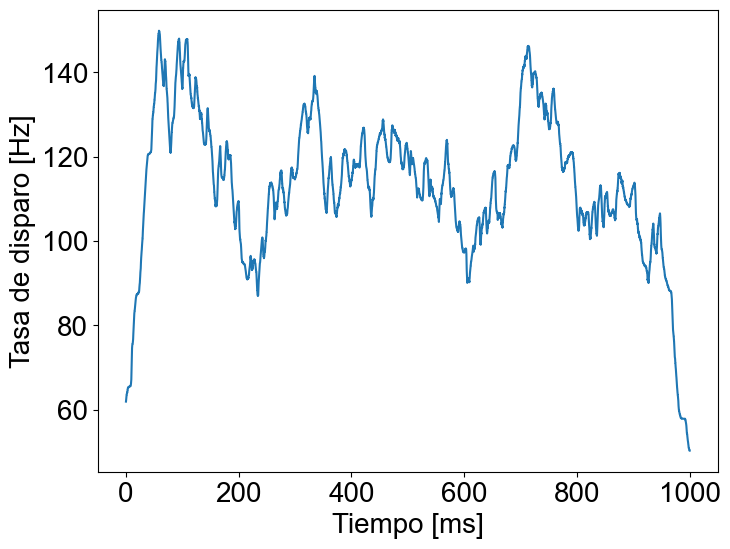
\includegraphics[width=\textwidth]{tasa_de_disparo_1000.png}
      \caption{\label{fig:tasa_de_disparo_1000}}
  \end{subfigure}
     \caption{Tasa de disparo para un ancho de caja de \ref{fig:tasa_de_disparo_2} $T = 2$ ms, \ref{fig:tasa_de_disparo_300} $T = 300$ ms y \ref{fig:tasa_de_disparo_1000} $T = 1000$ ms.}
     \label{fig:tasa_de_disparo}
\end{figure}

\section{Tasa de disparo}




Una herramienta útil para caracterizar la respuesta generada es la tasa de disparo, que se define como el número de spikes por unidad de tiempo. Esta tasa puede determinarse de dos maneras: promediando las señales de respuesta o, alternativamente, promediando el número de spikes en un intervalo temporal, o ''caja'', de ancho \(T\) para cada tiempo.

En este análisis, se eligió la segunda metodología. La tasa de disparo, calculada para diferentes anchos de caja \(T\), se presenta en la figura \ref{fig:tasa_de_disparo}. Se observa que el histograma es sensible al ancho \(T\) seleccionado. Con un \(T\) pequeño, como se observa en la figura \ref{fig:tasa_de_disparo_2}, la tasa refleja directamente las señales delta de los spikes. A medida que \(T\) se incrementa, la tasa de disparo revela información adicional, como se ve con \(T = 30\) ms en la figura \ref{fig:tasa_de_disparo_300}. Este comportamiento se mantiene en un amplio rango de $T$. Además, se observa un efecto de borde en los extremos temporales: la tasa decae notoriamente. Si \(T\) es excesivamente grande, como en la figura \ref{fig:tasa_de_disparo_1000}, el comportamiento general cambia debido a la pérdida de detalle de la información. Además, los efectos de borde se vuelven más notorios ya que el ancho de la caja se vuelve comparable con la duración total del intervalo de medición.


%Creo subfigura
\begin{figure}[h]
  \centering
  \begin{subfigure}[b]{0.35\textwidth}
      \centering
      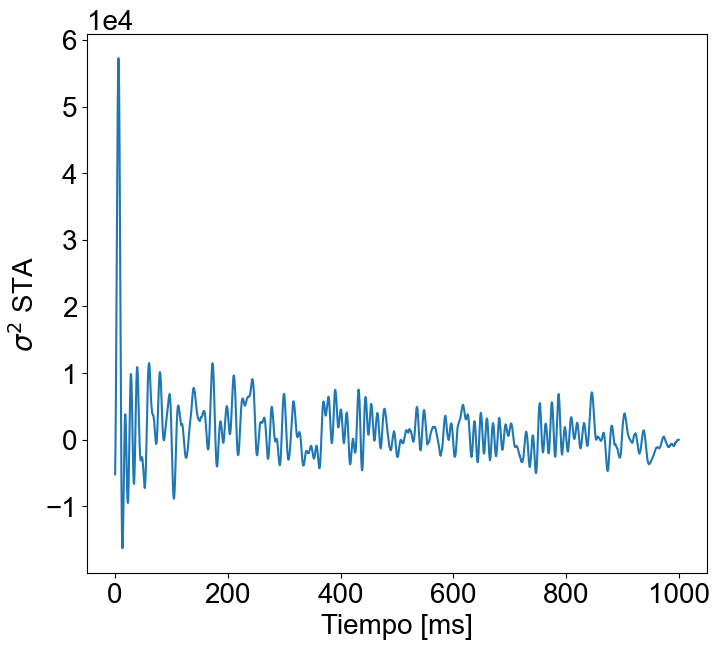
\includegraphics[width=\textwidth]{STA_total.png}
      \caption{\label{fig:STA_total}}
      \end{subfigure}
  \hfill
  \begin{subfigure}[b]{0.35\textwidth}
      \centering
      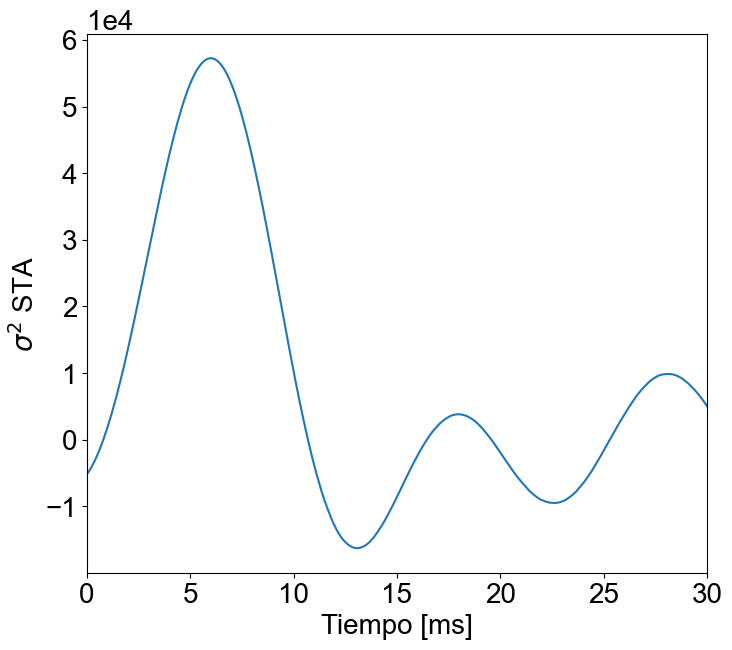
\includegraphics[width=\textwidth]{STA_parcial.png}
      \caption{\label{fig:STA_parcial}}
  \end{subfigure}
     \caption{Spike-Trigger-Average (STA) multiplicado por la constante de normalización $\sigma^2$ en función del tiempo $t$. En la figura \ref{fig:STA_total}, se grafica para todo el intervalo temporal, mientras que en la figura \ref{fig:STA_parcial} se grafica una ampliación para un intervalo menor.}
     \label{fig:STA}
\end{figure}

\begin{figure}[H]
  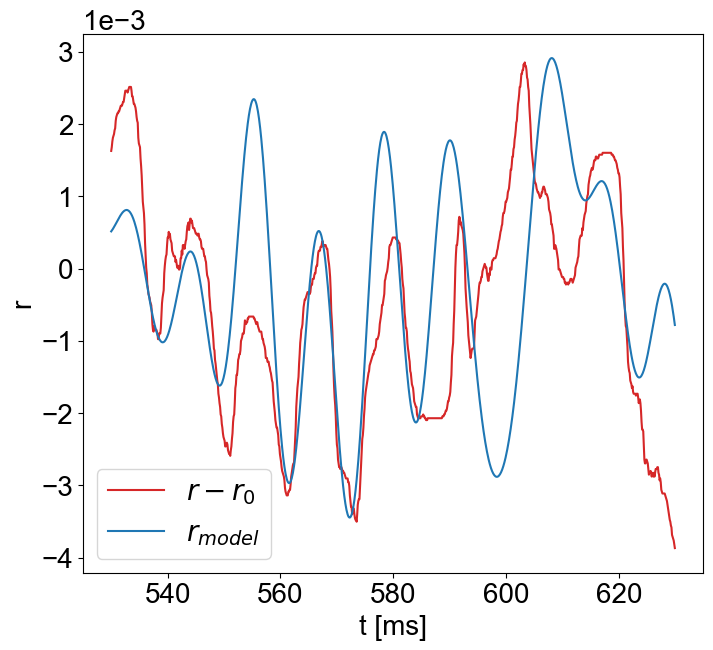
\includegraphics[clip=true,width=0.8\columnwidth]{r_vs_r_model.png}
  \caption{Diferencia en la tasa de disparo respecto a su valor medio $r - r_0$ y respuesta del modelo lineal $r_{model}$ adimensionalizada por $10^9$ en función del tiempo $t$.}
   \label{fig:r_vs_r_model}
\end{figure}

\section{Relación lineal entre estímulo y respuesta}

Hasta el momento, solo se ha caracterizado la respuesta neuronal. También resulta de gran interés estudiar la relación entre el estímulo presentado y la respuesta generada. Para entender tal relación, se puede considerar una descripción lineal de la respuesta en función del estímulo. Esta relación se puede expresar como

\[r(t) = r_0 + \int_0^\infty d\tau D(\tau) S(t - \tau)\]
donde \( r_0 \) es una constante y \( D(t) \) es una función denominada como kernel lineal.

Asumiendo que el valor medio del estímulo $S(t)$ es nulo, se obtiene que $r_0$ es el valor medio de la tasa de disparo, 116 Hz en este caso. Al despreciar el tiempo de autocorrelación del estímulo, el kernel lineal adquiere la forma
\[D(t) = \frac{1}{\sigma^2} \sum_{SPIKE} S(t_{SPIKE} - t).\]
Aquí, \( \sigma \) es una constante de normalización, $t_{SPIKE}$ es el tiempo al que ocurre un spike y la sumatoria se realiza sobre todos los spikes de todas las realizaciones. Con estas aproximaciones, el kernel lineal se conoce como Spike-Trigger-Average (STA).

El STA se presenta en función del tiempo en la figura \ref{fig:STA}. En esta figura, se destaca un pico para tiempos cortos alrededor de \( T_0 = 8 \) ms. Este sería el tiempo para el cual la neurona tiene mayor probabilidad de generar un spike tras un estímulo. Para tiempos más largos, el STA decae y muestra variabilidad, lo cual indica que la sensibilidad de la neurona disminuye con el tiempo.

Basándose en el STA, se calculó la respuesta  \( r_{model}(t) \) del modelo lineal. Para calcular la integral, se discretizó el tiempo y se limitó el intervalo de integración entre 0 y \( T_0 \) para evitar la variabilidad en \( D(t) \) para tiempos más largos. Consecuentemente, como se tiene la señal estímulo a partir de $t = 0$, se evaluó la respuesta a partir del tiempo \( t = T_0 \). Aunque sería necesario conocer la constante \( \sigma \) para comparar \( r(t) \) con \( r_{model}(t) \), se puede comparar \( r(t) - r_0 \) con \( r_{model}(t) \) adimensionalizado arbitrariamente por \( 10^9 \). Esta comparación se muestra en la figura \ref{fig:r_vs_r_model} para un rango limitado de tiempo usando una ventana temporal de 300 ms para calcular \( r(t) \). Se puede observar que el modelo captura aproximadamente el comportamiento de la respuesta, incluidos los picos y las depresiones, aunque presenta una gran variabilidad.


\onecolumngrid

\section{Apéndice}
A continuación se desarrolla el código empleado durante este trabajo implementado en Python.

\begin{lstlisting}[language=Python]
  #Import libraries
  import matplotlib.pyplot as plt
  import numpy as np
  
  #Import data .dat
  spikes = np.loadtxt('spikes.dat')
  stimulus = np.loadtxt('stimulus.dat')
  
  def ISI_calculation(realizacion):
      #Calculo los ISI de una realización realizacion es un vector de 0 y 1. Devuelve un vector con los ISI en unidades de 0.1 ms
      ISI = []
      index_last_spike = 0
      for i in range(1,len(realizacion)):
          if realizacion[i] == 1:
              ISI.append(i-index_last_spike)
              index_last_spike = i
      return np.array(ISI)
  
  def ISI_total_calculation(realizaciones):
      #Calculo los ISI de todas las realizaciones
      #realizaciones es una matriz de 0 y 1
      #Devuelve un vector con los ISI en unidades de 0.1 ms
      ISI = np.array([])
      for realizacion in realizaciones:
          ISI = np.concatenate([ISI, ISI_calculation(realizacion)])
      return ISI
  ISI_total = ISI_total_calculation(spikes)
  factor_to_ms = 1/10
  
  #Grafico el histograma normalizado de los ISI
  fig, ax = plt.subplots(1,1, figsize=(8,7))
  ax.hist(ISI_total*factor_to_ms, bins=100, density = True) #density=True
  ax.set_xlabel('ISI [ms]')
  ax.set_ylabel('P(ISI)')
  ax.set_xlim([0,40])
  plt.show()
  
  #Calculo media, desviación estandar y CV
  media = np.mean(ISI_total)
  desvio = np.std(ISI_total)
  CV = desvio/media
  print(f'Media: {media*factor_to_ms} [ms]')
  print(f'Desviación estandar: {desvio*factor_to_ms} [ms]')
  print(f'CV: {CV}')
  
  def N_calculation(realizaciones):
      #Calculo N. Devuelve un vector con los N
      return np.sum(realizaciones, axis=1)
  
  #Histograma de Ns normalizado
  fig, ax = plt.subplots(1,1, figsize=(8,7))
  ax.hist(N_calculation(spikes), bins=15) #density=True
  ax.set_xlabel('N')
  ax.set_ylabel('P(N)')
  plt.show()
  
  #Calculo media, desviación estándar y factor de Fano
  media = np.mean(N_calculation(spikes))
  desvio = np.std(N_calculation(spikes))
  Fano = desvio**2/media
  print(f'Media: {media}')
  print(f'Desviación estandar: {desvio}')
  print(f'Fano: {Fano}')
  
  def firing_rate_total_calculation(realizaciones, T):
      '''
      Calculo la tasa de disparo usando una caja de ancho T expresada en unidades de 0.1 ms, es decir, como índice. Tiene que ser múltiplo de 2
      '''
      N_realizaciones = len(realizaciones)
      return np.convolve(np.sum(realizaciones, axis = 0), np.ones(T), mode = "same")/T/N_realizaciones
  
  #Grafico la tasa de disparo
  def plt_tasa_de_disparo(T, save = False):
      fig, ax = plt.subplots(1,1, figsize=(8,6))
      y_vec = firing_rate_total_calculation(spikes[:,1:], T)/factor_to_ms*1e3
      x_vec = np.arange(len(y_vec))*factor_to_ms
      ax.plot(x_vec, y_vec)
      ax.set_xlabel('Tiempo [ms]')
      ax.set_ylabel('Tasa de disparo [Hz]')
      ax.set_title(f"Ancho de caja T = {T/10} ms")
      plt.show()
      if save == True:
          fig.savefig(f'tasa_de_disparo_{T}.png', bbox_inches='tight')
  
  plt_tasa_de_disparo(300, save = False)
  
  def t_spikes_calculation(realizacion):
      #Calculo los tiempos a los que se da un spike (t_spkies) de una realización
      #realizacion es un vector de 0 y 1
      #Devuelve un vector con los t_spikes en unidades de 0.1 ms
      tiempos = np.array(realizacion)*np.linspace(0, len(realizacion), len(realizacion))
      #Descarto tiempos nulos
      t_spike = tiempos[tiempos != 0]
      return t_spike
  
  def t_spikes_total_calculation(realizaciones):
      #Calculo los tiempos a los que se da un spike (t_spkies) de todas las realizaciones
      #realizaciones es una matriz de 0 y 1
      #Devuelve un vector con los t_spikes en unidades de 0.1 ms
      t_spike = np.array([])
      for realizacion in realizaciones:
          t_spike = np.concatenate([t_spike, t_spikes_calculation(realizacion)])
      return t_spike
  
  t_spikes_total = t_spikes_total_calculation(spikes)
  def kernel_lineal(t, t_spikes_total, stimulus_vec):
      '''
      Calcula D*sigma**2 expresado en unidades de dB
      t [0.1 ms]
      '''
      #Calculo la diferencia entre tiempos
      dif = t_spikes_total - t
      #Convierto el array de float a array de int
      dif = np.array(dif, dtype=int)
      #Elimino elementos negativos
      dif = dif[dif >= 0]
      #Evalúo S en dif como índices
      S_dif = stimulus_vec[dif]
      #Calculo D
      D = np.sum(S_dif)
      return D
  
  def kernel_constante(realizaciones):
      '''
      Calcula r0: valor medio de la tasa de disparo expresado en unidades de 1/0.1 ms
      '''
      return np.mean(realizaciones)
  
  #Calculo kernel_lineal y kernel_constante
  D_vec = np.empty(len(stimulus[:,0]))
  t_spikes_total = t_spikes_total_calculation(spikes)
  
  for i in range(len(stimulus[:,0])):
      D_vec[i] = kernel_lineal(i, t_spikes_total, stimulus[:,1])
  r0 = kernel_constante(spikes[:,1:])
  print(f"r0 = {r0/factor_to_ms*1e3} [Hz]")
  #Grafico D
  fig, ax = plt.subplots(1,1, figsize=(8,7))
  ax.plot(np.arange(len(stimulus[:,0]))*factor_to_ms, D_vec, color = "tab:blue")
  #Expreso el eje y en forma científica
  ax.ticklabel_format(axis="y", style="sci", scilimits=(0,0))
  # ax.plot(t_spikes_total)-
  ax.set_xlabel('Tiempo [ms]')
  ax.set_ylabel('$\sigma^2$ STA')
  plt.show()
  
  
  def modelo_lineal(r0, D_vec, stimulus_vec):
      '''
      Calcula la tasa de disparo r con el modelo lineal en función de r0, D_vec y stimulus. 
      r(t) = r0 + int_0^infty D(t')*stimulus(t-t')
      '''
      r_model = np.empty(len(stimulus_vec))
      Delta_t = factor_to_ms #Esta igualdad es una casualidad
      for t in range(len(stimulus_vec)):
          integral = 0
          T0 = 300 #[0.1 ms]. Límite superior de la integral
          if t < T0: #En esa regió no puedo hacer la integral
              r_model[t] = 0
          else: 
              for tau in range(T0):
                  integral += D_vec[tau]*stimulus_vec[t-tau]*Delta_t
              r_model[t] = integral
      return r_model
  
  r_model_vec = modelo_lineal(r0, D_vec, stimulus[:,1])
  #Grafico r y r_model
  fig, ax = plt.subplots(1,1, figsize=(8,7))
  T = 300
  r_vec = firing_rate_total_calculation(spikes[:,1:], T)
  
  ind_min = 0
  ind_max = 10000
  
  ax.plot(np.arange(len(r_vec))[ind_min:ind_max]*factor_to_ms, (r_vec - r0)[ind_min:ind_max], color = "tab:red", label = "$r - r_0$")
  ax.plot(stimulus[:,0][ind_min:ind_max], r_model_vec[ind_min:ind_max]/1e9, color = "tab:blue", label = "$r_{model}$")
  #Expreso eje y en forma científica
  ax.ticklabel_format(axis="y", style="sci", scilimits=(0,0))
  ax.set_ylabel('r')
  ax.set_xlabel('t [ms]')
  ax.legend()
  plt.show()
  

\end{lstlisting}

\bibliography{Chehade_practica_3.bib}

\end{document}





